\chapter{Relative Efficiency of Decoupled Adjoint Solver}
\label{chapter-nine}

At this point, the reacting gas adjoint in FUN3D has been utilized to obtain
sensitivity information needed to drive design optimization, and the
sensitivities of the fully coupled scheme have been validated against complex
frechet derivatives for accuracy.  A key point of this study is to demonstrate
the increase computational efficiency and relative memory saving of using a
decoupled variable set for the flow and adjoint solvers, instead of a fully
coupled variable set.  This chapter details the benefits of applying the
decoupled adjoint solver over the fully coupled solver for the annular jet
demonstration problem.

\section{Verification of Accuracy}

Section \ref{block-jacobi-decoupling} showed in detail that, in the adjoint,
changing from the fully coupled variable and equation sets to the decoupled
variable and equation sets could be accomplished by a series of matrix
transformations on the jacobian.  This transformation is equivalent to a left
and right preconditioning of the fully coupled scheme, enabling the reuse of the
approximate jacobians used by the flow solver.  Provided the adjoint system is
well conditioned and convergence is sufficient, preconditioning should not
affect the final adjoint solution; thus, we expect to recover the exact same
solution from both the fully coupled and decoupled adjoint schemes.

\section{Relative Memory Savings and Speedup}

The computational cost of the solution process in the adjoint can be greatly
improved by storing the exact linearizations of the discrete flow solver
equations, as discussed in \sref{sec:2nd-order-mem-cost}.  For a second order
scheme 
%------------------------------------------------------------------------------%
\begin{figure}[h]
	\begin{subfigure}[b]{0.45\textwidth}
    \centering
    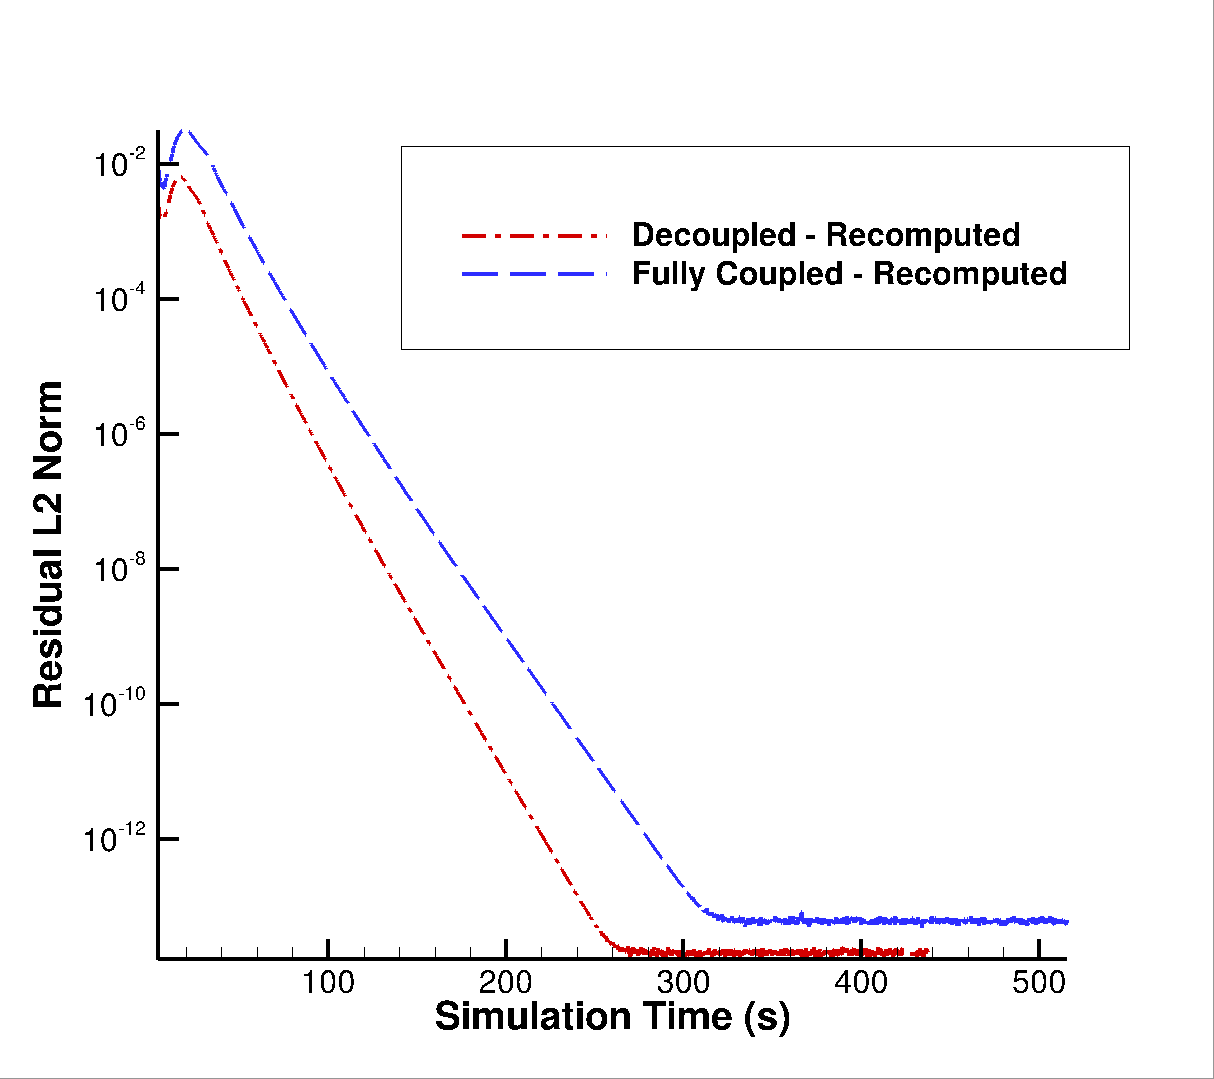
\includegraphics[width=\textwidth]{figures/adj-efficiency/adj-recompute.png}
    \caption{Linearizations Always Recomputed}
    \label{fig:always-recompute}
  \end{subfigure}
	\begin{subfigure}[b]{0.45\textwidth}
    \centering
    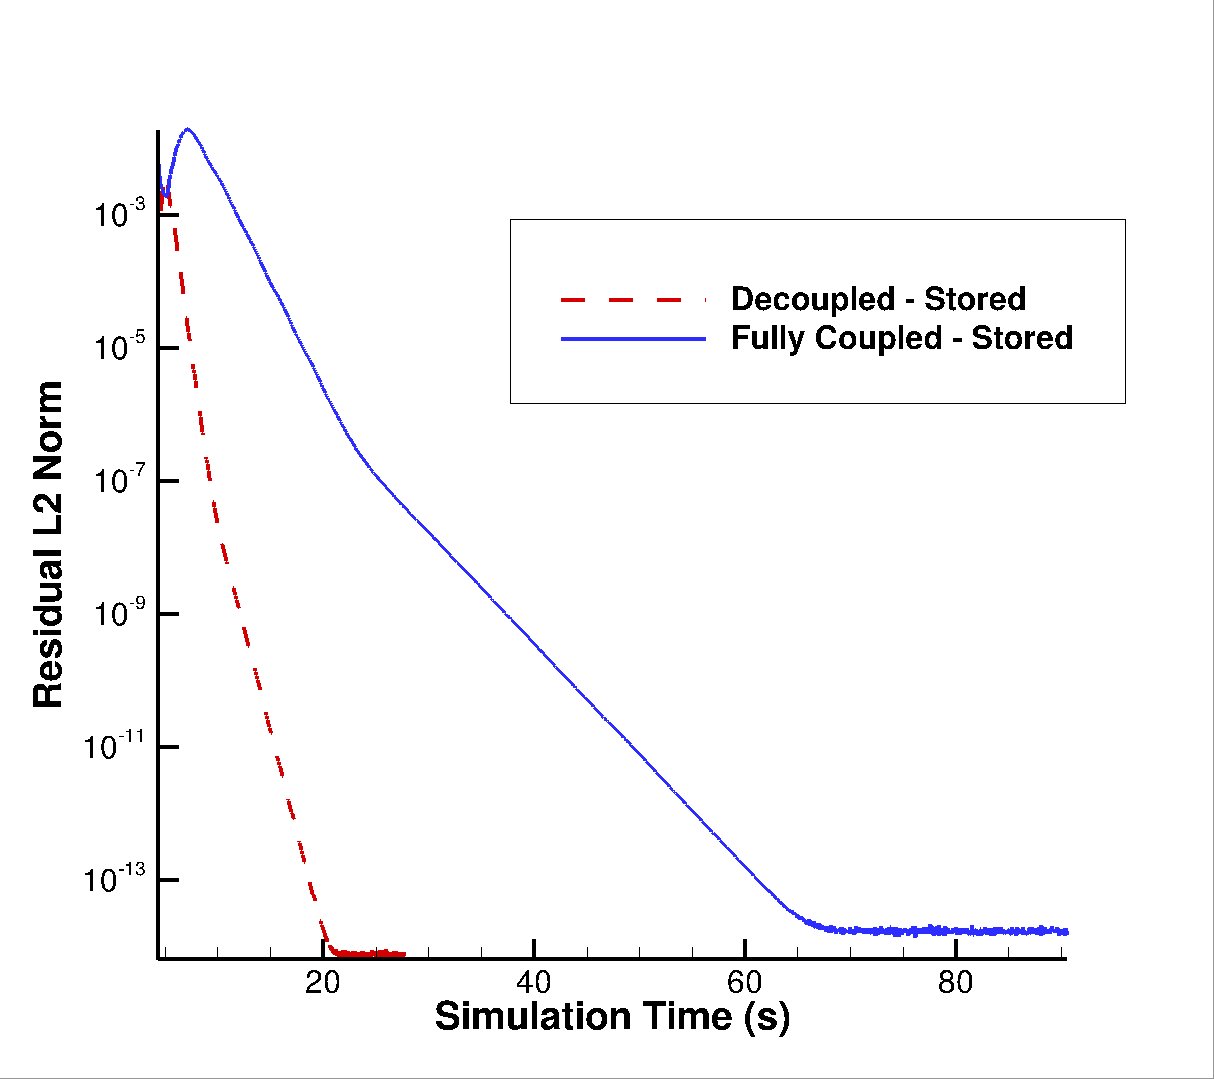
\includegraphics[width=\textwidth]{figures/adj-efficiency/adj-stored.png}
    \caption{Linearizations Stored}
    \label{fig:stored}
  \end{subfigure}
  \caption{Simulation Time Comparison}
  \label{fig:sim-time-comp}
\end{figure}
%------------------------------------------------------------------------------%
\fref{fig:sim-time-comp} shows the comparison of the fully coupled adjoint and 
decoupled adjoint time to solution with the two mechanisms for computing the
exact linearizations.  \tref{tab:srp-rel-speedup} shows that the speedup of
decoupled scheme is only truly realized when the exact linearizations are store,
rather than recomputed at each timestep. 
%------------------------------------------------------------------------------%
\begin{table}[h]
  \centering
  \begin{tabular}{c|c|c}
    Scheme & Time to Convergence (s) & Speedup \\
    \hline
    Fully Coupled (Recomputed Linearizations) & 309.4 & 1.0 (baseline)\\
    Decoupled (Recomputed Linearizations)     & 244.2 & 1.27 \\
    Fully Coupled (Recomputed Linearizations) & 61.22 & 5.05 \\
    Decoupled (Stored Linearizations)         & 18.69 & 16.6 \\
  \end{tabular}
  \caption{Relative Speedup}
  \label{tab:srp-rel-speedup}
\end{table}
%------------------------------------------------------------------------------%
This is because computing the exact linearizations in the adjoint is the
dominant cost.  The comparison between storing the linearizations and
recomputing them is somewhat unfair, as the ability to store the full jacobian
of the second order reconstruction may not be possible, due to memory
constraints.  That said, a significant advantage of the decoupled scheme over
the fully coupled scheme is the memory savings offered by the LHS jacobian
sparsity. It was show in \sref{sec:predicted-cost-mem-savings} that the
predicted memory savings for a infinite number of species is $1/7$ for a
hexahedral grid where the average number of neighbors is 6.  Unfortunately, the
storage requirements for the exact linearizations will not change between the
decoupled and fully coupled schemes; however, as the average number of neighbors
in the grid increases, the relative memory savings will also increase.  To
effectively demonstrate this, the amount of memory required by the adjoint
solver with the exact linearizations stored was determined for each mesh of the
refinement study in \sref{sec:mesh-refinement-study}.
%------------------------------------------------------------------------------%
\begin{figure}[h]
  \centering
	\begin{subfigure}[b]{0.45\textwidth}
    \centering
    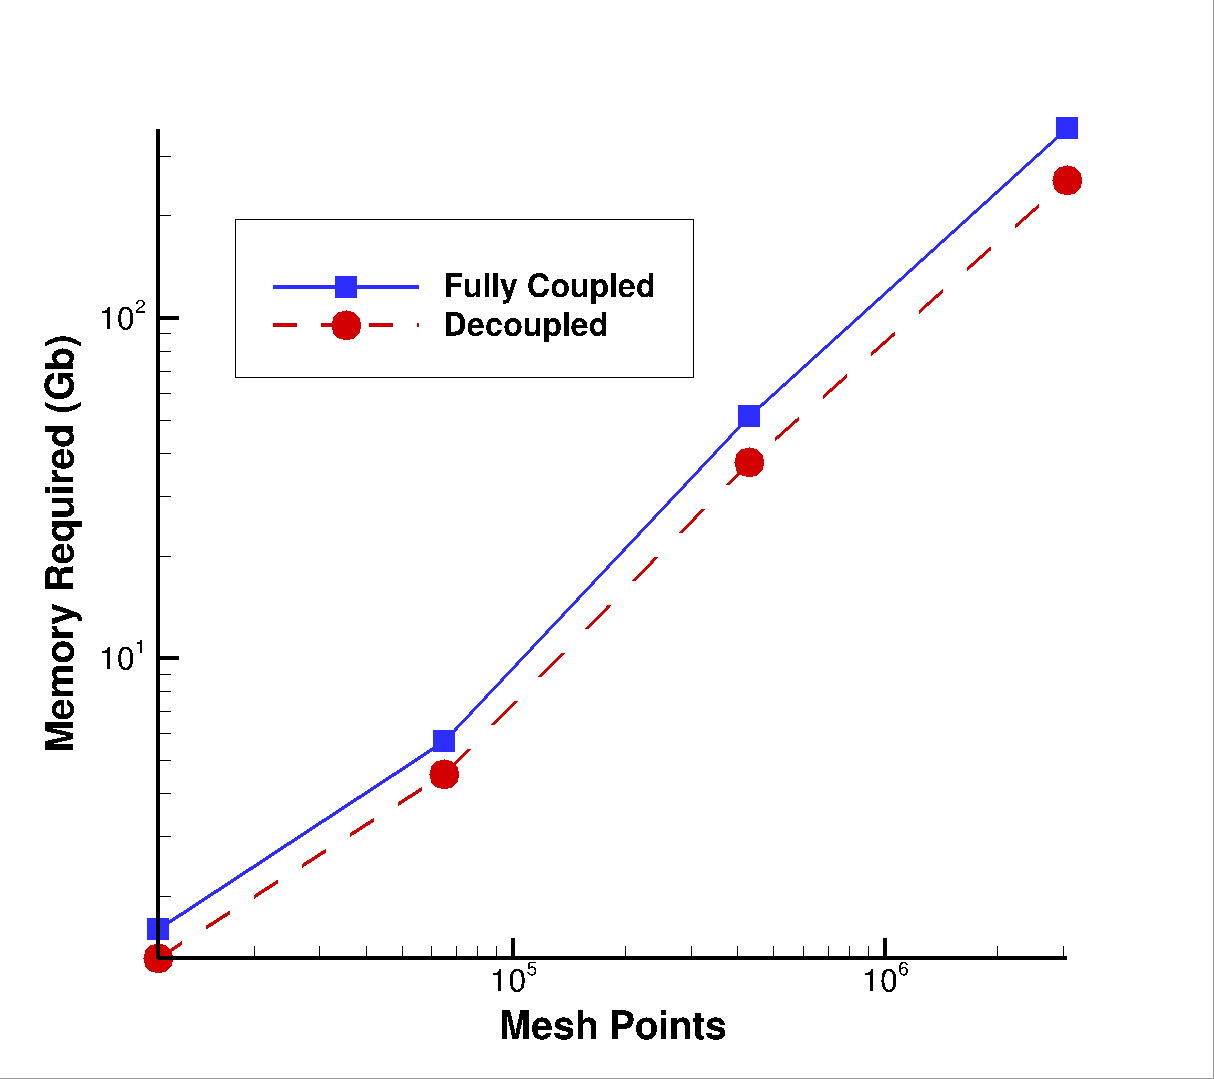
\includegraphics[width=\textwidth]{figures/adj-efficiency/mem-req-srp.png}
    \caption{Absolute Memory Required}
    \label{fig:abs-mem-req}
  \end{subfigure}
	\begin{subfigure}[b]{0.45\textwidth}
    \centering
    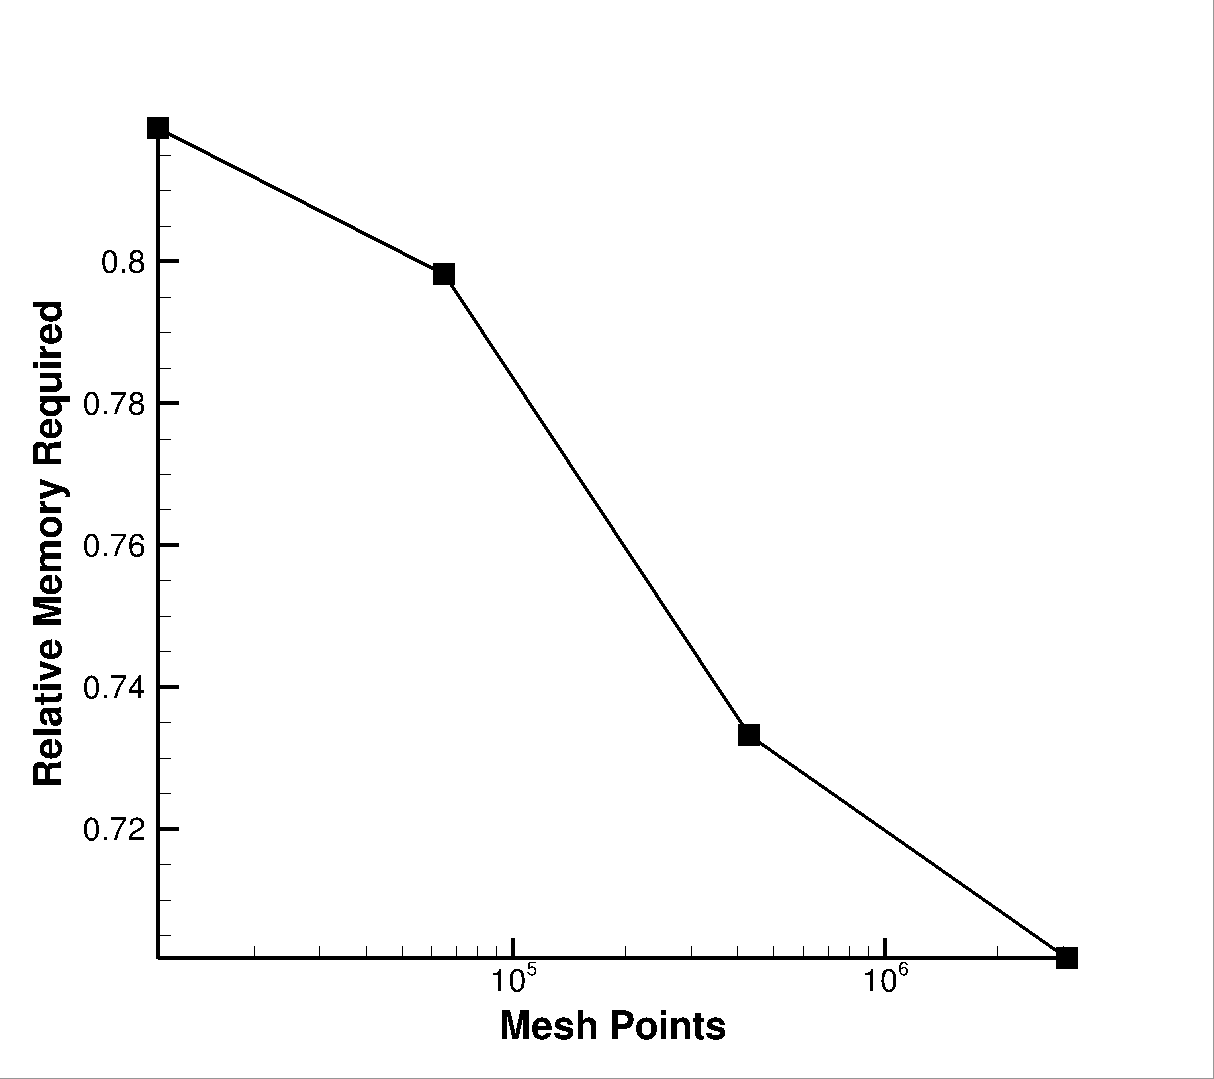
\includegraphics[width=\textwidth]{figures/adj-efficiency/mem-rel-savings.png}
    \caption{Relative Memory Required}
    \label{fig:relative-mem-req}
  \end{subfigure}
  \caption{Memory Required to Store Full Linearizations}
  \label{fig:srp-mem-req}
\end{figure}
%------------------------------------------------------------------------------%
\fref{fig:srp-mem-req} is somewhat encouraging a face value, since it was
possible to store the exact linearizations for the 3.1 million node mesh,
simulating a 9-species hydrogen air mixture.  \fref{fig:abs-mem-req} show, as
expected, that the memory requirements for both the fully coupled and decoupled
schemes scale directly with the number of mesh points.  The relative savings for
this case are nowhere near the predicted $1/7$ value, because the exact
linearizations require significantly more memory than anything else store in the
adjoint solver.  That said, the $\sim 20\%$ decrease in memory required by the
decoupled adjoint solver is significant, since the ability to store the exact
linearizations is a binary problem: either there is enough memory or there is
not.  The increased savings are as important as the speedup, if not more, since
the decoupled scheme can facilitate larger problems to be solved with greater
than an order of magnitude increase in computational efficiency.
